\documentclass[pdftex,12pt,a4paper]{article}

\usepackage{graphicx}  
\usepackage[margin=2.5cm]{geometry}
\usepackage{breakcites}
\usepackage{indentfirst}
\usepackage{pgfgantt}
\usepackage{pdflscape}
\usepackage{float}
\usepackage{epsfig}
\usepackage{epstopdf}
\usepackage[cmex10]{amsmath}
\usepackage{stfloats}
\usepackage{multirow}

\renewcommand{\refname}{REFERENCES}
\linespread{1.3}

% REQUIRED FOR INSETYING SOME SHITASS ASSEMBLY CODE INTO TO LATEX BIATCH fuck this retarded thing, science my ass
\usepackage{listings}
\usepackage{xcolor}
\definecolor{codegreen}{rgb}{0,0.6,0}
\definecolor{codegray}{rgb}{0.5,0.5,0.5}
\definecolor{codepurple}{rgb}{0.58,0,0.82}
\definecolor{backcolthe}{rgb}{0.95,0.95,0.92}
\definecolor{CommentGreen}{rgb}{0,.6,0}
% bu salak seyin son satiri bosluk olunca calismiyor kendimi sikcem simdi
% Icine comment de konmuyor

\lstset{
    numbers=left,
    basicstyle=\small\ttfamily,
    numberstyle=\tiny,
    keywordstyle=\color{blue}\bfseries,
    keywordsprefix=B,
    language={[x86masm]Assembler},
    breaklines=true,
    commentstyle=\color{codegreen},
    keywordstyle=\color{blue},
    keywordstyle=[2]\color{orange},
    keywordstyle=[3]\color{codegray},
    numberstyle=\tiny\color{codegray},
    stringstyle=\color{codepurple},
    showtabs=false,
    frame=single,
    keepspaces,
    escapechar=@,
}



\usepackage{mathtools}
%\newcommand{\HRule}{\rule{\linewidth}{0.5mm}}
\thispagestyle{empty}
\begin{document}
\begin{titlepage}
\begin{center}
\textbf{}\\
\textbf{\Large{ISTANBUL TECHNICAL UNIVERSITY}}\\
\vspace{0.5cm}
\textbf{\Large{COMPUTER ENGINEERING DEPARTMENT}}\\
\vspace{2cm}
\textbf{\Large{BLG 351E\\ MICROCOMPUTER LABORATORY\\ EXPERIMENT REPORT}}\\
\vspace{2.8cm}
\begin{table}[ht]
\centering
\Large{
\begin{tabular}{lcl}
\textbf{EXPERIMENT NO}  & : & 1 \\
\textbf{EXPERIMENT DATE}  & : & 02.10.2019 \\
\textbf{LAB SESSION}  & : & WEDNESDAY - 13.30 \\
\textbf{GROUP NO}  & : & G10 \\
\end{tabular}}
\end{table}
\vspace{1cm}
\textbf{\Large{GROUP MEMBERS:}}\\
\begin{table}[ht]
\centering
\Large{
\begin{tabular}{rcl}
150170062  & : & Mehmet Fatih YILDIRIM \\
150180704  & : & Cihat AKK\.{I}RAZ \\
150180705  & : & Batuhan Faik DER\.{I}NBAY \\
150180707  & : & Fatih ALTINPINAR \\
\end{tabular}}
\end{table}
\vspace{2.8cm}
\textbf{\Large{FALL 2019-2020}}

\end{center}

\end{titlepage}

\newpage


\thispagestyle{empty}
\addtocontents{toc}{\contentsline {section}{\numberline {}FRONT COVER}{}}
\addtocontents{toc}{\contentsline {section}{\numberline {}CONTENTS}{}}
\setcounter{tocdepth}{4}
\tableofcontents
\clearpage

\setcounter{page}{1}


\section{INTRODUCTION}
% microcontrollers diye düzelttim. gerçi cümle kendisi de 1az şeymiş, which ekledim
One of the microcontrollers from Texas Instruments family is MSP430 which is a mixed signal microcontroller. The MSP430 is designed for low cost and specifically low power consumption. This is the first of the experiments in this period, a simple introduction to the MSP430 was made. In this experiment, MSP430 microcontroller is programmed in order to achieve LED on-off patterns on the experiment booklet. 

\section{MATERIALS AND METHODS}

This experiment is completed by using a MSP430G2553 microprocessor. This microprocessor is programmed by using Code Composer Studio for the desired tasks on the experiment handout. During coding several sources are used:

\begin{itemize}
    \item MSP430 Education Board Manual \cite{ref2}
    \item MSP430 Architecture Chapter 4 \cite{ref3}
    \item MSP430 Instruction Set \cite{ref4}
\end{itemize}

\subsection{Part 1}
 
\newline{}
In the first part of the experiment, a new CCS Project is created as choosing "MSP430G2553" as the target and "Empty Assembly Project" as the project template. Then, code given on the experiment booklet \cite{booklet}(see Figure \ref{code:part1}) is put to the main.asm file.
For better understanding, further examination of the code, line by line if necessary is required:

\begin{itemize}
    \item Line 1: P1.0 is enabled for future use.
    \item Line 2: P1.0 is complemented via using XOR instruction to flash.
    \item Line 3 - 5: This is the wait function. The value $250000_{10}$ is moved to register 15 and decreased on the 4th line. Taking the 5th line into hand, until the zero flag is raised the program jumps back to 4th line, decreasing the value of R15. When the value in R15 hits $0_{10}$, the zero flag is raised causing line 5 to skip execution and continuum of the program.
    \item Line 6: In order to flash the LED the program jumps to main loop(Seen in 2)
\end{itemize}
%\begin{lstlisting}[language={[x86masm]Assembler}, numbers=left]

\begin{figure}[H]
    \centering
    \begin{lstlisting}[label={code:part1}]
SetupP1     bis.b   #001h,  &P1DIR 
Mainloop    xor.b   #001h,  &P1OUT 	 
Wait        mov.w   #250000,R15 	 
L1          dec.w   R15 			 
            jnz L1				 
            jmp Mainloop		 
    \end{lstlisting}
    \label{code:part1}
    \caption{Assembly Code of Part 1}
\end{figure}

\subsection{Part 2}
In the second part of the experiment, the microprocessor was programmed to flash the LEDs as in the given pattern(see Figure \ref{fig:part2}).

\begin{figure}[H]
    \centering
    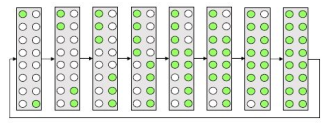
\includegraphics[width=0.75\textwidth]{part2.png}
    \caption{Part 2 LEDs On - Off Pattern}
    \label{fig:part2}
\end{figure}

In order to implement the given pattern, team created following piece of code given in Figure \ref{code:part2}

\begin{figure}[H]
    \centering
    \begin{lstlisting}[language={[x86masm]Assembler}]
SetupP2		mov.b 	#0FFh,	&P1DIR 	 
		mov.b	#0FFh,	&P2DIR 	 
Reset		mov.b	#01h,	&P1OUT 	 
		mov.b	#80h,	&P2OUT 	 
		jmp 	Wait 			 

Mainloop	rla.b	&P1OUT 			 
		add.b 	#01h,	&P1OUT 	 
		rra.b	&P2OUT 			 
Wait		mov.w 	#250000,R15 	 
L1		dec.w	R15 			 
		jnz 	L1				 
		cmp.b	#0FFh, 	P2OUT	 
		jz      Reset    
		jmp 	Mainloop     
    
    \end{lstlisting}
    \label{code:part2}
    \caption{Assembly Code of Part 2}
\end{figure}

For better understanding, further examination of the code, line by line if necessary, is required:

\begin{itemize}
    \item Line 1: The first column of LEDs are set up. Notice that all LEDs in the first column will be needed, as clearly seen at the last state in Figure \ref{code:part2}. The binary representation for this case would be $11111111_2$. Therefore, in this line, the value $11111111_2\;(0xFF)$ is moved to the absolute address $P1DIR$ in order to activate all LEDs in the first column.

    \item Line 2: For the exact same reasons, namely, because of the need for all LEDs to light up, in this line, the value $11111111_2\;(0xFF)$ is moved to the absolute address $P2DIR$ in order to activate all LEDs in the second column.

    \item Line 3-5: This is the Reset function that will later be used to reach the first state in Figure \ref{code:part2}. In line 3, the value $00000001_2\;(0x01)$ is moved to the absolute address  $&P1OUT$ in order to light the first LED in the first column. Similarly, in line 4, the value $10000000_2\;(0x80)$ is moved to the absolute address  $&P2OUT$ in order to light the last LED in the second column. Note that the least significant bit (LSB) is located at the top of the column and the most significant bit (MSB) is located at the bottom of the column. In line 5, the program jumps to the Wait function.

    \item Line 7-9: This is the Mainloop that will be executed in order to achieve the next state. In line 7, the value at the address $&P1OUT$ is arithmetically shifted to left in order to light the next LED. In line 8, this value in $&P1OUT$ is incremented by 1 in order to light the first LED in first column again which went of in line 7. In line 9, the value at the address $&P2OUT$ is arithmetically shifted to right in order to light the next LED. Since "arithmetically" shifted, the leftmost digit corresponding to the last LED in second column will automatically filled with 1 which was the value here before shifting. Therefore, an operation like the one in line 8 is not needed.

    \item Line 10-12: This is the Wait function that will be executed in order to provide the delay between each 2 consecutive states. In line 10, the value $250000_{10}$ is moved to register 15 and in line 11, it is decreased. In line 12, until the zero flag is raised the program jumps back to 11th line to decrease the value in R15. When the value in R15 hits $0_{10}$, the zero flag is raised and the program skips to the next line.

    \item Line 13-15: In line 13, the value at $&P2OUT$ is compared with $11111111_2\;(0xFF)$ in order to know whether all LEDs in second column are lit which means the last state is reached. If they are equal, the zero flag is raised. In line 14, if it is raised, the program jumps to Reset function to reach the first state again. In line 15, the program jumps to Mainloop to achieve the next state because if this line is reached, it is known that the last state is not reached yet.
\end{itemize}

\newpage
\subsection{Part 3}
\newline{}
In the part 3 of the first experiment the LED's were lit in a descending order, changing the column every two steps as shown in Figure \ref{fig:part3}.
\paragraph{}
In order to achieve the given sequence the team decided on the following piece of code given in Figure \ref{code:part3}.
For better understanding, further examination of the code, line by line if necessary, is required:
\begin{itemize}
    \item Line 1: The first of line of LEDs are set up. Notice the pattern that starting with two LEDs, every second doublet of LEDs will be lit. When sketched, "$O$" denoting LEDs that are needed to be lit and "$X$" that don't need to be lit, the pattern can be expressed as "$XXOOXXOO$" for the first line of LEDs. Hence the binary representation of such expression will be "$00110011_2$". Note that the least significant bit (LSB) is located at the top of the column and the most significant bit (MSB) is located at the bottom of the column.
    \newline
    Therefore in this line the value $00110011_2\;(0x33)$ is moved to the absolute address $P1DIR$ in order to activate aforementioned LEDs.
    \item Line 2:Since the LEDs that will be lit in the second column follow the "$OOXXOOXX$", $11001100_2\;(0xCC)$ value is moved the absolute address $P2DIR$ in the second line.
    \item Line 3: This is the reset function. $00000001_2\;(0x01)$ is stored in register 14 in order to set the initial state of the LEDs.
    \item Line 4-5: This is the beginning of the main loop. The value in R14 is moved the absolute addresses of LEDs in order to light them. Notice that every value of R14 is moved to both LED columns but each LED will light up according to the "SetupP3" when certain values are present.
    \item Line 6:The value in the register 14 is arithmetically shifted to left in order to light the next LED. For a better representation binary expressions can be checked up on. For example the very first value stored in R14 ($00000001_2$) results in ($00000010_2$) after an arithmetic shift left.
    \item Line 7-9: This is the wait function. The value $250000_{10}$ is moved to register 15 and decreased on the 8th line. Taking the 9th line into hand, until the zero flag is raised the program jumps back to 8th line, decreasing the value of R15. When the value in R15 hits $0_{10}$, the zero flag is raised causing line 9 to skip execution and continuum of the program.
    \item Line 10-12: 10th line checks whether the 8bit value in register 14 is $0_{10}\;(0x00)$ or not. If that's the case, the zero flag is raised and the program jumps to "Reset" function as depicted on line 11. If the zero flag is not raised this means that not all 8 rows of LEDs were lit, hence the program jumps to main loop (Seen in line 12) in order to light up the next LED in the sequence.
\end{itemize}

\begin{figure}[H]
    \centering
    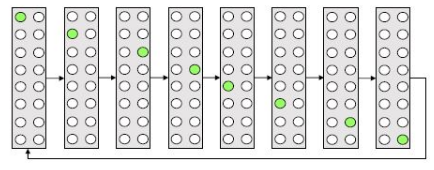
\includegraphics[width=0.75\textwidth]{part3.png}
    \caption{Part 3 LEDs On - Off Pattern}
    \label{fig:part3}
\end{figure}

\begin{figure}[H]
    \centering
\begin{lstlisting}[language={[x86masm]Assembler}, numbers=left]
SetupP3         mov.b   #033h, 	&P1DIR  
                mov.b 	#0CCh, 	&P2DIR  
Reset		mov.b	#01h, 	R14  
Mainloop	mov.b 	R14,	&P1OUT	 
                mov.b	R14, 	&P2OUT	 
                rla.b	R14				 
Wait		mov.w 	#250000,R15  
L1              dec.w	R15  
                jnz     L1 
                cmp.b	#000h,  R14 
                jz      Reset  
                jmp     Mainloop 
\end{lstlisting}
    \caption{Assembly Code of Part 3}
    \label{code:part3}
\end{figure}


% yaw bussuru olay var da cok kanserler gercekten hayattan soguttu beni kodun o programdaki fotosunu atsana renklerine bakcam 
% rakkkamlar turuncuydu galiba da onu yapamadim registerlarin bide labellerin rengi var mi
% Code composera gir bak ben evdeki pcdeyim burda kurulu degil
% ama ne kadar renkli o kadar pro duruyo :D
%  bende d eyok senin pc de kapali ha gerci raporda ornegi var dimi
% var benim laptop cantamda\
% salla gitsin xd ilk experimentttan bak renklndir yav seqilli shuqullu olsun

\subsection{Part 4}

\begin{figure}[H]
    \centering
    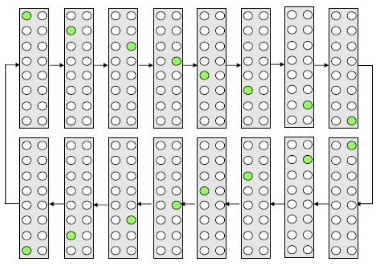
\includegraphics[width=0.75\textwidth]{part4.png}
    \caption{Part 4 LEDs On - Off Pattern}
    \label{fig:part4}
\end{figure}

\newline{}
In the final part of the experiment, a modification is required to be applied on Part 3's code in order to achieve the sequence in Part 4.
\paragraph{}
As can be seen in Figure \ref{fig:part4}, in the second part of the sequence only the LEDs that are on the opposite side will light up. To achieve this, the values of $P1DIR$ and $P2DIR$ have to be swapped. This can be done by adding lines from 4 to 7 to the code and changing line 16. Rather than jumping back to Reset like in Figure \ref{code:part3}, jumping to SetupB is required to initiate the second part of the sequence.

\newline{}
Line by line explanation of the SetupF sequence is required in order to have a better understanding:

\begin{itemize}
    \item Line 4-5: Since first and second parts of the sequence given in Figure \ref{fig:part4} should cycle over time, the code should be returning to first part of the sequence after completing the second. This is achieved by these lines.  $P2DIR$ is checked, if its equal to $00110011_2$ which means that it is in the second part of the sequence, then zero flag will be up. Line 5, will initiate the SetupF.
    \item Line 6-5; Since LEDs have to lit on the opposite way, values of $P1DIR$ and $P2DIR$ are swapped.
\end{itemize}



% In the final part of the experiment, LED's were lit in a descending order, changing the column every two steps and as shown in Figure \ref{fig:part4}.
% \newline{} % Ben report2 ye başlıyorum hem anlamış olurum daha iyi kodları o zaman
% In order to achieve the given sequence the team decided on the following piece of code given in Figure \ref{code:part4}

% \newline{}




% \begin{itemize}
% \item T
%      %cihat part 4 ü bana sal abi ben onu batununkinin ütüne kurup yazarım xd
%      % sen part1 i anlat ordaki koddan ne anladınız diye de soruyolar part2 yi de mfy yaspın inş
%      %tamamdır reis :)
     
%      % sa xd
%      % abi herşeyi size kitledim de onu ayip oldu valla
%      % her satiri eklemiyelim bak ben halledeyim soyle diyelim
%      % part3 ek olarak 2. sequence i elde etmek icin enable olanlarin yerini degistirmemiz gerekiyordu onu degistirmek icin su satirlari ekledik diye yaparsak yeterli olur bence
%      % Olabilir aynı 
% \end{itemize}
% %Ne kitlemesi hiçbişey yapmıyoz :S asıl size ayıp oldu

\newline{}

\begin{figure}[H]
    \centering
\begin{lstlisting}[language={[x86masm]Assembler}, label={code:part4}, caption={}]
SetupF		mov.b	#033h,	&P1DIR	 
			mov.b	#0CCh,	&P2DIR	 
			jmp 	Reset			 
SetupB		cmp.b	#033h,	&P2DIR	 
			jz		SetupF			 
			mov.b	#0CCh,	&P1DIR	 
			mov.b	#033h,	&P2DIR	 
Reset		mov.b	#01h, 	R14 	 
Main		mov.b 	R14,	&P1OUT	 
			mov.b	R14, 	&P2OUT	 
			rla.b	R14				 
Wait		mov.w 	#250000,R15 	 
L1			dec.w	R15 			 
			jnz 	L1				 
			cmp.b	#000h,	R14		 
			jz 		SetupB			 
			jmp 	Main			 
\end{lstlisting}
    \caption{Assembly Code of Part 4}
    \label{code:part4}
\end{figure}


\section{RESULTS}%conc kısmı niye benim cümlelerim  
There wasn't any problem or any unexpected situations. Results were observed the way the team has predicted them. Desired LEDs on - off patterns and the codes to implement these patterns are given in the previous section.

\section{DISCUSSION}

\newline{}
Preparing the code before going to the lab session speeds up the team's work. In the lab session, the code was debugged to correct minor errors. There was no contradiction between the theoretical knowledge of the team and the results of the experiment.
\newline
Please refer to section 2 "MATERIALS AND METHODS" for exclusively detailed information, tables, images, analysis, interpretation and results, covering all the required material under other sections.

%Please explain, analyze, and interpret what have you done during the  experiment. 
\newpage
\section{CONCLUSION}
%It was not difficult at all. We just nailed it goddamnit.
Team didn't face any particular difficulties that were worth noting throughout the experiment. Team was able to complete the given tasks quite swiftly. All in all, this experiment helped team members to improve their abilities to program MSP430 microprocessor for given conditions situations.

% Discussion a mi alsak o cumleyi?
%sen bilirsin knk takil kafana gore
\nocite{overleaf}
\nocite{reportGuide}
\newpage
\addcontentsline{toc}{section}{\numberline {}REFERENCES}

\bibliographystyle{unsrt}
\bibliography{reference}

\end{document}

